\documentclass{article}
\usepackage[sexy, hdr, fancy]{evan}
\setlength{\droptitle}{-4em}

\lhead{Homework 7}
\rhead{Introduction to Statistics}
\lfoot{}
\cfoot{\thepage}

\newcommand{\var}{\mathrm{Var}}
\newcommand{\cov}{\mathrm{Cov}}

\begin{document}
\title{Homework 7}
\maketitle
\thispagestyle{fancy}

\begin{enumerate}
	\item[1.] Suppose an iid vector of data $\underline{X}=(X_1,\cdots, X_n)$ can belong to one of two classes $Y,$ where $Y=0$ or $Y=1.$ A \textit{decision rule} or \textit{classifier} $g$ is a function $g:\RR^n\to \RR$ that assigns to any $n$-tuple of data a value 0 or 1. Suppose that the so-called \textit{class conditional} densities $f_0$ and $f_1$ of $\underline{X}$ are given, \[f_j(x_1, \cdots, x_n)=f(x_1, \cdots, x_n\mid Y=j), \quad j=0, 1\] are given. Define $L^0(g)$ and $L^1(g)$ as follows: \[L^0(g) = P(g(\underline{X})=1\mid Y=0), \quad L^1(g) = P(g(\underline{X})=0\mid Y=1)\] For $c>0,$ define the decision rule \[g_c(x_1, \cdots, x_n)=\begin{cases}
				1 \text{ if } cf_1(x_1, \cdots, x_n)>f_0(x_1,\cdots, x_n) \\
				0\text{ otherwise}
		\end{cases} \] Prove that for any classifier $g,$ if $L^0(g)<L^0(g_c),$ then $L^1(g)>L^1(g_c).$ In other words, if $L^0$ is required to be kept under a certain level, then the decision rule minimizing $L^1$ has the form $g_c$ for some $c.$
		\begin{proof}
			Since $g_c(\underline{X})$ and $g(\underline{X})$ are Bernoulli random variables, the condition $L^0(g)<L^0(g_c)$ means that
			\begin{align*}
				P_0(g(X)=1) &< P_0(g_c(X)=1) \\
				\tag{1}E_0[g(X)] &< E_0[g_c(X)]
			\end{align*}
			Consider the inequality \[g_c(X)\left[ c f_1(X)-f_0(X) \right]\ge g(X)\left[ c f_1(X)-f_0(X) \right]\] If $g_c(X)=1,$ then $cf_1(X)>f_0(X)$ so the LHS is positive. If $g(X)=1$ then the two sides are equal, and if $g(X)=0,$ then the LHS is greater. If $g_c(X)=0,$ then $cf_1(X)\le f_0(X),$ so the RHS is either 0 or non-positive, while the LHS is 0. 

			If we integrate both sides over all possible $X,$ using the fact that $\int g_c(X) f_1(X) = E[g_c(X)\mid Y=1] = E_1[g_c(X)]$ and etc, we have
			\begin{align*}
				c E_1[g_c(X)] - E_0[g_c(X)] &\ge c E_1[g(X)] - E_0[g(X)] \\
				E_0[g(X)]-E_0[g_c(X)] &\ge c\left( E_1[g(X)]-E_1[g_c(X)] \right) \\
				E_0[g_c(X)]-E_0[g(X)] &\le c\left( E_1[g_c(X)]-E_1[g(X)] \right) \\
			\end{align*}

			From (1), the LHS is positive, so the RHS is positive as well. Thus, \[E_1[g_c(X)]>E_1[g(X)]\] and since these are Bernoulli random variables, we have
			\begin{align*}
				P_1(g_c(X)=1) &> P_1(g(X)=1) \\
				1-P_1(g_c(X)=0) &> 1-P_1(g(X)=0) \\
				P_1(g(X)=0) &> P_1(g_c(X)=0) \\
				L^1(g) &> L^1(g_c)
			\end{align*}
			as desired.
			
		\end{proof}

	\item[2.] Suppose we consider a Bayesian framework for hypothesis testing, in which we consider testing a simple null vs a simple alternative: \[H_0: \mu=\mu_0, \quad H_a: \mu=\mu_a\] Suppose we have the probabilities $P(\mu=\mu_0)$ and $P(\mu=\mu_a)$ as the \textit{prior probabilities} that the null or alternative are true. Suppose we are given a distribution of the data under both null and alternative, so that \[f(x_1, \cdots, x_n\mid \mu=\mu_0), \quad f(x_1, \cdots, x_n\mid \mu=\mu_a)\] are given. How would you use the prior and likelihood to construct a test of hypothesis. Be completely specific about your test statistic and how it is computed.
		\begin{soln}
			We have the posterior ratio \[\frac{P(H_0\mid \underline{X})}{P(H_a\mid \underline{X})}=\frac{P(H_0)}{P(H_a)}\cdot \frac{f(\underline{X}\mid H_0)}{f(\underline{X}\mid H_a)}\] If this ratio is greater than 1, we choose $H_0,$ and otherwise, we choose $H_a.$ Thus, we have \[\frac{f(\underline{X}\mid H_0)}{f(\underline{X}\mid H_a)}>\frac{P(H_a)}{P(H_0)}\] as the likelihood ratio test. We know the prior probabilities, so this is a valid test.
			
		\end{soln}
		
	\item[11.] Suppose $X_1, \cdots, X_n$ are iid standard normal data. Show that the vector of random variables given by $(X_1-\bar{X}, \cdots, X_n-\bar{X})$ is independent of $\bar{X}$ for the case $n=2.$ Use this independence for more general $n$ to show that for any sample size $n,$ the scaled sample variance $(n-1)s^2$ is the sum of squares of independent standard normal random variables.
		\begin{proof}
			Consider the joint density of $(X_1-\bar{X}, \bar{X}).$ Since $X_i$ are normal random variables, these are just linear combinations of normal random variables, thus they are both normal. Then the covariance is 
			\begin{align*}
				\cov(X_1-\bar{X}, \bar{X}) &= E[(X_1-\bar{X})\bar{X}] - E[X_1-\bar{X}]E[\bar{X}] \\
				&= E[X_1 \bar{X}] - E[\bar{X}^2] = E\left[ X_1 \cdot \frac{1}{n} \sum_{i=1}^{n} X_i \right] - \left(E[\bar{X}^2]-(E[\bar{X}]^2) \right)- (E[\bar{X}])^2  \\
				&= \frac{1}{n} \sum_{i=1}^{n} E[X_1 X_i] - \var(\bar{X}) \\
				&= \frac{1}{n} \left( E[X_1^2] + \sum_{i=2}^{n}E[X_1]E[X_i] \right)-\frac{1}{n} \\
				&= \frac{1}{n} \left( \var(X_1) + (E[X_1])^2 \right) - \frac{1}{n} = \frac{1}{n} \left( 1 \right)-\frac{1}{n} = 0
			\end{align*}
			Since this is a pair of bivariate normal random variables, and their covariance is zero, it follows that they are independent. Thus, by extension, the entire vector is independent of $\bar{X},$ as desired.

			We have the scaled sample variance \[(n-1)s^2 = \sum_{i=1}^{n} (X_i-\bar{X})^2\] Each of $X_i-\bar{X}$ is a standard normal random variable, and they are each independent, so we are done.

		\end{proof}

\end{enumerate}

\section*{Chapter 9: Hypothesis Testing and Assessing Goodness of Fit}

\begin{itemize}
	\item[10.] Suppose that $X_1, \cdots, X_n$ form a random sample from a density function, $f(x\mid \theta),$ for which $T$ is a sufficient statistic for $\theta.$ Show that the likelihood ratio test of $H_0:\theta=\theta_0$ vs $H_A:\theta=\theta_1$ is a function of $T.$ Explain how, if the distribution of $T$ is known under $H_0,$ the rejection region of the test may be chosen so that the test has the level $\alpha.$
		\begin{proof}
			Since $T$ is a sufficient statistics, we can factor the likelihood as \[f(X_1, \cdots, X_n\mid \theta) = g(T, \theta) h(X_1, \cdots, X_n)\] Thus, the likelihood ratio test is given by
			\begin{align*}
				\Lambda &= \frac{f(X_1,\cdots, X_n\mid \theta=\theta_0)}{f(X_1, \cdots, X_n\mid \theta=\theta_1)} = \frac{g(T, \theta_0) h(X_1, \cdots, X_n)}{g(T, \theta_1) h(X_1, \cdots, X_n)} \\
				&= \frac{g(T, \theta_0)}{g(T, \theta_1)} = h(T)
			\end{align*}
			since $\theta_0$ and $\theta_1$ are just constant values, this ratio is only a function of $T,$ as desired.

			$\Lambda$ is just some function of $T,$ and we can find the probability \[P(\Lambda\le c\mid H_0) = P(h(T)\le c\mid H_0)=\alpha\] This probability only depends on the null distribution of $T$ supposing we can invert $h$ (or even if it is not invertible). Thus, if we are given $\alpha,$ we can solve for the value of $c,$ and thus the rejection region corresponds with $\Lambda=h(T)\le c$ for which we can solve for values of $T$ that we would reject.

		\end{proof}

	\item[12.] Let $X_1, \cdots, X_n$ be a random sample from an exponential distribution with the density function $f(x\mid \theta)=\theta\exp(-\theta x).$ Derive a likelihood ratio test of $H_0:\theta=\theta_0$ vs $H_A:\theta\neq \theta_0,$ and show that the rejection region is of the form $\left\{ \bar{X}\exp(-\theta_0 \bar{X})\le c \right\}.$
		\begin{soln}
			The MLE of the exponential distribution is given by $\hat{\theta}=1/\bar{X}.$ The GLR is given by
			\begin{align*}
				\Lambda &= \frac{f(X_1, \cdots, X_n\mid \theta=\theta_0)}{f(X_1, \cdots, X_n\mid \theta=1/\bar{X})} = \frac{\prod_{i=1}^{n}\theta_0 e^{-\theta_0 X_i}}{\prod_{i=1}^{n}\frac{1}{\bar{X}}e^{-X_i/\bar{X}}} \\
				&= (\theta_0 \bar{X})^n \exp\left[ -\left(\theta_0-\frac{1}{\bar{X}}\right)\sum_{i=1}^{n} X_i \right] \\
				&= (\theta_0 \bar{X})^n \exp\left[ -\left( \theta_0-\frac{1}{\bar{X}}\right) n\bar{X}\right] \\
				&= (\theta_0 \bar{X})^n \exp\left[ n-n\theta_0 \bar{X} \right] \\
				&= \theta_0^n e^n \left( \bar{X} \exp\left( -\theta_0 \bar{X} \right) \right)^n
			\end{align*}
			Since we reject this for small $\Lambda,$ the rejection region is defined by the set
			\begin{align*}
				\Set{\underline{X}}{\Lambda\le c} &= \Set{\underline{X}}{\theta_0^n e^n \left( \bar{X}\exp\left( -\theta_0 \bar{X} \right) \right)^n\le c} \\
				&= \left\{ \underline{X}\mid \bar{X}\exp(-\theta_0 \bar{X}) \le \frac{c^{1/n}}{\theta_0 e}\right\} \\
			\end{align*}
			as desired.

		\end{soln}

	\item[13.] Suppose, to be specific, that in Problem 12, $\theta_0=1, n=10,$ and that $\alpha=0.05.$ In order to use the test, we must find the appropriate value of $c.$
		\begin{enumerate}[a.]
			\item Show that the rejection region is of the form $\left\{ \bar{X}\le x_0 \right\}\cup \left\{ \bar{X}\ge x_1 \right\},$ where $x_0$ and $x_1$ are determined by $c.$
				\begin{proof}
					We have \[\Lambda=e^n (\bar{X}\exp(-\bar{X}))^n\le c\] so \[\bar{X}\exp(-\bar{X})\le \frac{c^{1/10}}{e}\] is the rejection region. The plot of the LHS is shown below:
					\begin{center}
						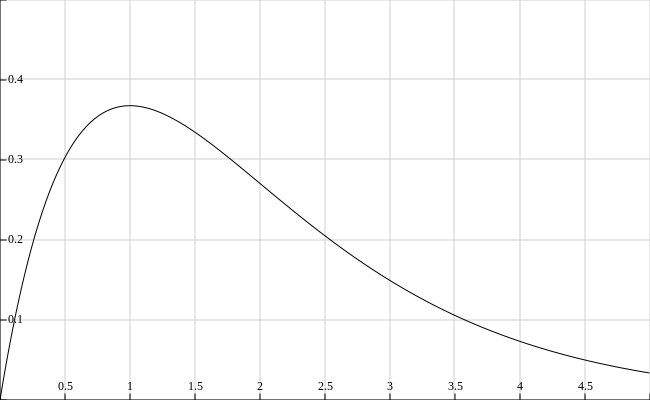
\includegraphics[width=10cm]{save.png}
					\end{center}
					which shows that any horizontal line through this graph (a threshold) intersects twice, and the solution region is a union of two intervals of the form desired. The endpoints of these intervals depends on the horizontal line chosen, which corresponds to whatever $c^{1/10}/e$ is.

				\end{proof}

			\item Explain why $c$ should be chosen so that $P(\bar{X}\exp(-\bar{X})\le c)=0.05$ when $\theta_0=1.$
				\begin{answer*}
					We are in the significance level $\alpha=0.05,$ so $c$ should be chosen so the probability of type I error is 0.05.
				\end{answer*}

			\item Explain why $\displaystyle \sum_{i=1}^{10} X_i$ and hence $\bar{X}$ follow gamma distributions when $\theta_0=1.$ How could this knowledge be used to choose $c?$
				\begin{answer*}
					The sum of independent exponential random variables follows a Gamma distribution. Thus, we can explicitly determine the distribution of $Y=\bar{X} \exp(-\bar{X})$ (although this isn't nicely solvable, theoretically it would be) so we can figure out $c$ so that \[P(Y\le c)=0.05\]
				\end{answer*}

			\item Suppose that you hadn't thought of the preceding fact. Explain how you could determine a good approximation to $c$ by generating random numbers on a computer.
				\begin{answer*}
					Generate 10 exponential random variables with $\theta=1,$ compute $\bar{X} \exp(-\bar{X}).$ Run this simulation many times, storing each trial. The mean of all the trials should be approximately normal by the Central Limit Theorem, so $P(\bar{X}\exp(-\bar{X})\le c)=\alpha$ and we must find the value of $c$ such that this is 0.05, which is easy if we standardize.
				\end{answer*}
				
		\end{enumerate}

	\item[14.] Suppose that under $H_0,$ a measurement $X$ is $N(0, \sigma^2),$ and that under $H_1, X$ is $N(1, \sigma^2)$ and that the prior probability $P(H_0)=2P(H_1).$ The hypothesis $H_0$ will be chosen if $P(H_0\mid x)>P(H_1\mid x).$ For $\sigma^2=0.1, 0.5, 1.0, 5.0:$
		\begin{enumerate}[a.]
			\item For what values of $X$ will $H_0$ be chosen?
				\begin{soln}
					We choose $H_0$ if 
					\begin{align*}
						\frac{P(H_0\mid x)}{P(H_1\mid x)}&=\frac{P(H_0)}{P(H_1)}\cdot \frac{f(x\mid H_0)}{f(x\mid H_1)} = 2\cdot \frac{f(x\mid H_0)}{f(x\mid H_1)}>1\\
						\implies\frac{f(x\mid H_0)}{f(x\mid H_1)}&>\frac{1}{2} \\
					\end{align*}
					We have
					\begin{align*}
						\frac{\frac{1}{\sqrt{2\pi}\sigma}\exp\left( -\frac{x^2}{2\sigma^2} \right)}{\frac{1}{\sqrt{2\pi}\sigma}\exp\left( -\frac{(x-1)^2}{2\sigma^2} \right)} &= \exp\left( -\frac{1}{2\sigma^2}\left[ x^2-(x-1)^2 \right] \right) \\
						&= \exp\left( -\frac{2x-1}{2\sigma^2} \right) >\frac{1}{2}
					\end{align*}
					Solving for $x,$ we find \[x<\frac{1}{2}+\sigma^2\ln 2\] are the values of $x$ for which we choose $H_0.$ To find the values of $X$ for which we choose $H_0$ at various values of $\sigma^2,$ just substitute in.
					
				\end{soln}

			\item In the long run, what proportion of the time will $H_0$ be chosen if $H_0$ is true 2/3 of the time?
				\begin{answer*}
					In the long run, we expect to choose $H_0$ approximately 2/3 of the time.
				\end{answer*}
				
		\end{enumerate}

	\item[18.] Let $X_1, \cdots, X_n$ be iid random variables from a double exponential distribution with density \[f(x)=\frac{1}{2}\lambda \exp(-\lambda\abs{x}).\] Derive a likelihood ratio test of the hypothesis $H_0:\lambda=\lambda_0$ vs $H_1:\lambda=\lambda_1$ where $\lambda_0$ and $\lambda_1>\lambda_0$ are specified numbers. Is the test uniformly most powerful against the alternative $H_1:\lambda>\lambda_0?$
		\begin{soln}
			We have the likelihood ratio
			\begin{align*}
				\Lambda &= \frac{f(X_1, \cdots, X_n\mid \lambda=\lambda_0)}{f(X_1, \cdots, X_n\mid \lambda=\lambda_1)} = \frac{\displaystyle\prod_{i=1}^{n} \frac{1}{2}\lambda_0 \exp(-\lambda_0\abs{X_i})}{\displaystyle\prod_{i=1}^{n} \frac{1}{2}\lambda_1 \exp(-\lambda_1\abs{X_i})} \\
				&= \left( \frac{\lambda_0}{\lambda_1} \right)^n \exp\left[ -(\lambda_0-\lambda_1)\sum_{i=1}^{n} \abs{X_i} \right] \le c \\
				\sum_{i=1}^{n}\abs{X_i} &\le \frac{1}{\lambda_1-\lambda_0}\log\left[ c\left( \frac{\lambda_1}{\lambda_0} \right)^n \right]
			\end{align*}
			Since $H_0$ and $H_1$ are simple hypotheses, the Neyman-Pearson Lemma guarantees this will be most powerful. For the alternative $H_1:\lambda>\lambda_0,$ since $\lambda_1>\lambda_0$ for any simple alternative in this case, and this likelihood ratio is most powerful for each, it is uniformly most powerful against $H_1:\lambda>\lambda_0.$
			
		\end{soln}

	\item[20.] Consider two PDFs on [0, 1]: $f_0(x)=1$ and $f_1(x)=2x.$ Among all tests of the null hypothesis $H_0:X\sim f_0(x)$ versus the alternative $X\sim f_1(x),$ with significance level $\alpha=0.10,$ how large can the power possibly be?
		\begin{soln}
			Since these are simple null and simple alternative, by the Neyman-Pearson Lemma, the likelihood ratio test is most powerful, so we use that. We have
			\begin{align*}
				\Lambda &= \frac{f(X\mid X\sim f_0)}{f(X\mid X\sim f_1)} = \frac{1}{2X} \\
			\end{align*}
			so the likelihood ratio test at significance level $\alpha=0.10$ is 
			\begin{align*}
				P(\Lambda\le c\mid H_0) &= \alpha=0.10 \\
				P\left( \frac{1}{2X} \le c \bigg\vert X\sim f_0 \right) &= P\left( X\ge \frac{1}{2c}\bigg\vert X\sim f_0 \right) \\
				&= 1-\frac{1}{2c} = 0.10 \\
				\implies c &= \frac{5}{9}
			\end{align*}

			Thus, the power is given by
			\begin{align*}
				P(\Lambda\le c\mid H_1) &= P\left( \frac{1}{2X}\le \frac{5}{9}\bigg\vert X\sim f_1 \right) \\
				&= P\left(X\ge \frac{9}{10} \bigg\vert X\sim f_1\right) \\
				&= \int_{9/10}^1 \frac{1}{2x} \, dx = 1-\left( \frac{9}{10} \right)^2 = 0.19
			\end{align*}
			and this is maximal, as guaranteed by the Neyman-Pearson Lemma.

		\end{soln}

	\item[24.] Let $X$ be a binomial random variable with $n$ trials and probability $p$ of success.
		\begin{enumerate}[a.]
			\item What is the GLR for testing $H_0:p=0.5$ vs $H_A:p\neq 0.5?$
				\begin{soln}
					For the MLE, we consider the log-likelihood and its derivative wrt $p:$
					\begin{align*}
						\log f(X=x\mid p) &= \log\left[ \binom{n}{x} p^{x}(1-p)^{n-x} \right] \\
						&= \log \binom{n}{x} + x\log p + (n-x)\log (1-p) \\
						\frac{\partial}{\partial p} \log f(X=x\mid p) &= \frac{x}{p}-\frac{n-x}{1-p} = 0 \\
						p &= \frac{x}{n}
					\end{align*}
					Thus, the GLR is given by
					\begin{align*}
						\Lambda &= \frac{f(X=x\mid p=0.5)}{f(X=x\mid p=x/n)} = \frac{\binom{n}{x}\left( \frac{1}{2} \right)^n}{\binom{n}{x} \left( \frac{x}{n} \right)^x\left( 1-\frac{x}{n} \right)^{n-x}} \\
						&= \left( \frac{1}{2} \right)^n \left( \frac{n}{x} \right)^x \left( \frac{n}{n-x} \right)^{n-x} = \left( \frac{n/2}{x} \right)^x \left( \frac{n/2}{n-x} \right)^{n-x}
					\end{align*}
				\end{soln}

			\item Show that the test rejects for large values of $\abs{X-n/2}.$
				\begin{proof}
					We have
					\begin{align*}
						\Lambda &= \left( \frac{n}{2x} \right)^x \left(\frac{n}{2(n-x)}\right)^{n-x} \\
						&= \left( \frac{1}{\frac{2x}{n}} \right)^x \left( \frac{1}{2\left( 1-\frac{x}{n} \right)} \right)^{n-x} \\
						&=\left[ \left( \frac{2x}{n} \right)^{-2x/n}\left(2-\frac{2x}{n}  \right)^{-2+2x/n} \right]^{n/2} 
					\end{align*}
					Let $y=2x/n,$ so this becomes \[\Lambda = \left[y^{-y} \left( 2-y \right)^{2-y}\right]^{n/2}\] Let $z = 1-y.$ Then we have \[\Lambda = \left[ (1-z)^{-(1-z)}(1+z)^{-(1+z)} \right]^{n/2}\] Note that this is symmetric about $z=0$ (obvious, let $z'=-z$ and the two values are exactly equal) so this is symmetric about $2x/n=1.$ It also attains its maximum value at $z=0$ (first and second derivative tests omitted). Thus, if we are far from $z=0,$ we reject the since then $\Lambda$ is small. This is equivalent to a large value of \[\abs{\frac{2x}{n}-1}=\frac{2}{n}\abs{x-\frac{n}{2}}\] so if $\abs{x-n/2}$ is large, we reject the null, as desired.

				\end{proof}

			\item Using the null distribution of $X,$ show how the significance level corresponding to a rejection region $\abs{X-n/2}>k$ can be determined.
				\begin{soln}
					The null distribution is \[P(X=x)=\binom{n}{x} \left( \frac{1}{2} \right)^n\] Thus, we have
					\begin{align*}
						\alpha &= P(\abs{X-n/2}>k\mid H_0) = P(X-n/2>k) + P(n/2-X > k) \\
						&= P(X > k+n/2) + P(X < n/2 - k)
					\end{align*}
					To compute this, just sum the PMF from the null distribution over the values in the rejection region.
					
				\end{soln}

			\item If $n=10$ and $k=2,$ what is the significance level of the test?
				\begin{soln}
					From above, we have
					\begin{align*}
						\alpha &= P(X>2+10/2) + P(X<10/2-2)= P(X > 7) + P(X < 3) \\
						&= \left(\frac{1}{2}\right)^{10}\left[ \binom{10}{8}+\binom{10}{9}+\binom{10}{10} + \binom{10}{0}+\binom{10}{1}+\binom{10}{2} \right] \\
						&= \frac{7}{64}
					\end{align*}
				\end{soln}

			\item Use the normal approximation to the binomial distribution to find the significance level if $n=100$ and $k=10.$
				\begin{soln}
					A binomial distribution with $n$ trials and probability $p$ is approximately \[N\left( np, np(1-p) \right) = N\left( 50, 5^2 \right)\] in this case. Thus, the significance level is
					\begin{align*}
						\alpha &= P(X > 10+100/2) + P(X<100/2 - 10) = P(X > 60) + P(X < 400) \\
						&= P\left( \frac{X-50}{5} > 2 \right) + P\left( \frac{X-50}{5} < -2 \right) \\
						&\approx 2\Phi(-2) \approx 0.0455
					\end{align*}
				\end{soln}
				
		\end{enumerate}

	\item[26.] True or false:
		\begin{enumerate}[a.]
			\item The generalized likelihood ratio statistic $\Lambda$ is always less than or equal to 1.
				\begin{answer*}
					This is true. The likelihood in the denominator is the max over all possible values of a parameter, which is always greater than or equal to the max over a subset of the possibilities.
				\end{answer*}

			\item If the $p$-value is 0.03, the corresponding test will reject at the significance level 0.02.
				\begin{answer*}
					This is false. The test will only reject if the $p$-values is less than the significance level.
				\end{answer*}

			\item If a test rejects at a significance level 0.06, then the $p$-value is less than or equal to 0.06.
				\begin{answer*}
					This is true. We reject as $p$-values less than the significance level.
				\end{answer*}

			\item The $p$-value of a test is the probability that the null hypothesis is correct.
				\begin{answer*}
					This is false. The $p$-value is the smallest significance level at which we reject the null hypothesis.
				\end{answer*}

			\item In testing a simple versus simple hypothesis via the likelihood ratio, the $p$-value equals the likelihood ratio.
				\begin{answer*}
					This is false. The $p$-value is not the likelihood ratio, it is a probability.
				\end{answer*}

			\item If a chi-square test statistic with 4 degrees of freedom has a value of 8.5, the $p$-value is less than 0.05.
				\begin{answer*}
					This is false. The $p$-value in this case is 0.07.
				\end{answer*}
				
		\end{enumerate}

	\item[30.] Suppose that the null hypothesis is true, that the distribution of the test statistic, $T$ say, is continuous with CDF $F$ and that the test rejects for large values of $T.$ Let $V$ denote the $p$-value of the test.
		\begin{enumerate}[a.]
			\item Show that $V=1-F(T).$
				\begin{proof}
					Suppose we reject if $T>M$ for some $M.$ The $p$-value is defined as \[V=P(T\ge M\mid H_0)=1-P(T<M\mid H_0) = 1-F(T)\] as desired.
					
				\end{proof}

				\newpage
			\item Conclude that the null distribution of $V$ is uniform. (Hint: Prop C Section 2.3)
				\begin{soln}
					Since $F$ is a CDF, it is increasing and invertible. Thus, we have 
					\begin{align*}
						P(V\le v) &= P(1-F(T)\le v) = P(F(T)\ge 1-v) \\
						&= P(T\ge F\inv(1-v)) = 1-P(T<F\inv(1-v)) \\
						&= 1-F(F\inv(1-v)) = 1-(1-v) = v
					\end{align*}
					So the density of $V$ is the derivative of this wrt $v,$ which is 1, so $V$ is uniform on the interval [0, 1], as desired.

				\end{soln}

			\item If the null hypothesis is true, what is the probability that the $p$-value is greater than 0.1?
				\begin{answer*}
					Since $V$ follows a uniform distribution, $P(V>0.1)=0.9.$
				\end{answer*}

			\item Show that the test that rejects if $V<\alpha$ has significance level $\alpha.$
				\begin{proof}
					Since $V=P(T>M\mid H_0),$ we have $P(T>M\mid H_0)<\alpha.$ At the significance level $\alpha,$ we reject $H_0$ if this probability is less than $\alpha,$ which is true in this case. Thus, we will reject $H_0,$ as desired.
					
				\end{proof}
				
		\end{enumerate}
		
\end{itemize}

\end{document}
